\section{Introduction}\label{sec:intro}

Objects in the real world rarely exist in isolation; understanding and modeling the relationships between them is essential to accurately capturing complex systems. As increasingly powerful machine learning models progress towards building internal ``world models,'' a crucial frontier of research is exploring natural inductive biases which enable efficient learning of relational representations. The computational challenge lies in developing the components necessary for constructing robust, flexible, and progressively complex relational representations.

% Modeling of relations between objects is important to a range of machine learning problems. For instance, an image analysis application might rely on comparing objects in terms of relations that extract color, size, or texture features; a natural language task may use relations that are based on syntactic or semantic features of pairs of words. To enable efficient learning of relational information, it is important to explore learning architectures that support processing of relations in a natural, expressive, and efficient manner.

Compositionality---the ability to compose modules together to build iteratively more complex feature maps---is key to the success of deep representation learning. For example, in a feed forward network, each layer builds on the one before, and in a CNN, each convolution builds an iteratively more complex feature map~\citep{zeiler2014visualizing}. So far, work on relational representation learning has been limited to ``flat'' first-order architectures. In this work, we propose a compositional framework for learning hierarchical relational representations, which we call ``relational convolutional networks.''

A schematic of the proposed architecture is shown in~\Cref{fig:relconv_architecture}. The key idea involves formalizing a notion of ``convolving'' a relation tensor, describing the pairwise relations in a sequence of objects, with a ``graphlet filter'' which represents a template of a relational pattern between groups of objects. Each composition of those operations computes relational features of a higher order---i.e., relations on relations.

\begin{wrapfigure}{R}{0.5\textwidth}
    \vskip -20pt
    \centering
    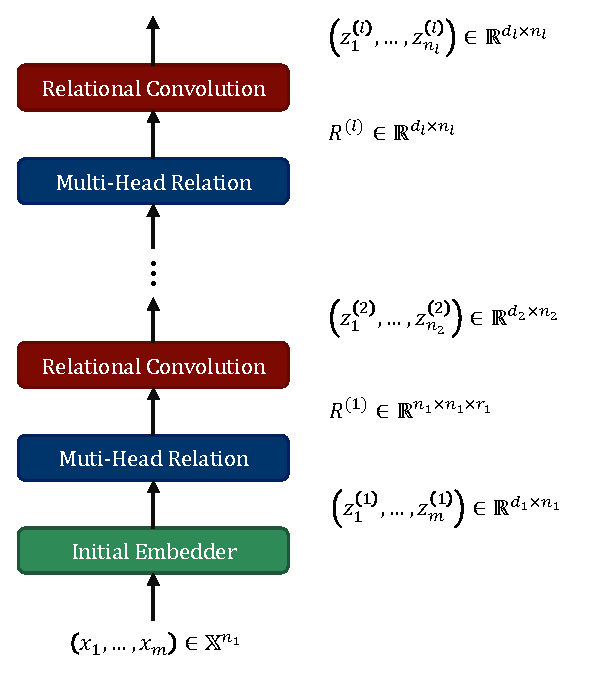
\includegraphics[width=.5\textwidth]{figs/relconv_architecture.pdf}
    \vskip-5pt
    \caption{Proposed architecture for relational convolutional networks. Hierarchical relations are modeled by iteratively computing pairwise relations between objects and convolving the resultant relation tensor with graphlet filters representing templates of relations between groups of objects.
    }\label{fig:relconv_architecture}
\end{wrapfigure}

In a series of experiments, we show how relational convolutional neural networks provide a powerful framework and inductive bias for relational learning. We first carry out experiments on ``relational games'' proposed as a benchmark for relational reasoning by~\citep{shanahanExplicitlyRelationalNeural}. This consists of a suite of binary classification tasks for identifying abstract relational rules between a set of objects represented as images. We next carry out experiments on a version of the SET game, which requires processing of higher-order relations between multiple attributes on a set of cards. For both tasks, relational convolutional networks are able to achieve more sample efficient learning compared to Transformers, as well as other architectures that have been specifically developed for relational learning.

\subsection{Related Work}

Several previous works have considered the design of machine learning architectures which support the representation of relational information, in various forms~\citep{battagliaRelationalInductiveBiases2018,palmRecurrentRelationalNetworks2018,zhangRAVENDatasetRelational2019}.

\textbf{Graph Neural Networks.} Graph neural networks (GNNs) are a class of neural network architectures which operate on graphs and process ``relational'' data~\citep{niepertLearningConvolutionalNeural2016,kipfSemiSupervisedClassificationGraph2017,schlichtkrullModelingRelationalData2017,velickovicGraphAttentionNetworks2017,kipfNeuralRelationalInference2018}. A defining feature of the GNN model is its use of a form of neural message-passing, wherein the hidden representation of a node is updated as a function of the hidden representations of its neighbors~\citep{gilmerNeuralMessagePassing2017}. Typical examples of tasks which GNNs are applied to include node classification, graph classification, and link prediction~\citep{hamiltonGraphRepresentationLearning2020}. %This is a very general model which includes as a special case convolutional neural networks, where the graph is a grid, and Transformers, where the graph is a complete graph and the message-passing function is a convex sum of the neighbors' representations. In our experiments, we compare to Transformers as a representative of the GNN model.

In GNNs, the `relations' are given to the model via edges in a graph. In contrast, our architecture, as well as the explicitly relational architectures described below, operate on collections of objects without any relations given as input. Instead, such relational architectures must infer the relevant relations from the objects themselves. Still, graph neural networks can be applied to relational tasks by passing in the collection of objects along with a complete graph. A Transformer Encoder can be thought of as a special case of this architecture, and hence is the representative baseline we compare against in our experiments.

\textbf{Attention as modeling relations} Several works have proposed architectures with the ability to model relations by incorporating an attention mechanism~\citep{vaswani2017attention,locatelloObjectCentricLearningSlot2020,santoroRelationalRecurrent2018,zambaldiDeepReinforcementLearning2018,velickovicGraphAttentionNetworks2017}. Attention mechanisms model relations between objects implicitly as an intermediate step in a form of neural message-passing in order to update the representation of each object as a function of its context.

\textbf{Emerging literature on ``explicitly relational'' architectures.} There exists a growing literature on neural architectures which aim to explicitly model relational information between objects. An early example is~\citep{santoroSimpleNeural2017}.~\citet{shanahanExplicitlyRelationalNeural} proposes the PrediNet architecture, which aims to learn relational representations which are compatible with predicate logic.~\citet{webbEmergentSymbols2021} proposes ESBN, a recurrent neural network augmented with external memory with a memory-write operation which factors representations into `sensory' and `relational'.~\citet{kergNeuralArchitecture2022} proposes CoRelNet, a simple architecture based on `similarity scores' which aims to distill the relational inductive biases discovered in previous work into a minimal architecture. %CoRelNet is shown to perform favorably compared to ESBN and PrediNet on the tasks considered in those papers.

We aim to contribute to this literature by proposing a framework for learning hierarchical relational representations in a natural, interpretable, sample-efficient, and parameter-efficient manner.